\section{Математическе модели}

    В данном разделе представленно описание модели частотного скана 
    в математических выражениях.


    \subsection{Модель сигнала релаксации ёмкости}

    Согласно обзору \cite{istratov_exp_analysis}, зависимость значения
    ёмкости от времени $f(t)$ для моноэкспоненциального сигнала релаксации
    имеет вид выражения \ref{eq:monoexp}.
    \begin{equation}
        \label{eq:monoexp}
        f(t) = A \exp \left(-\lambda t\right) ,
    \end{equation}
    где
    \begin{description}
        \item[\(A\)] -- амплитуда сигнала релаксации ёмкости;
        \item[\(\lambda\)] -- скорость экспоненциального спада,
        обратнопрпорциональная постоянной веремени сигнала релаксации
        $\tau$ (выражение \ref{eq:lambda}).
    \end{description}
    \begin{equation}
        \label{eq:lambda}
        \lambda = \tau ^ {-1}
    \end{equation}
    Спектр моноэкспоненциального сигнала релаксации имеет вид, 
    представленный на рисунке \ref{pic:monoexp_spect_example}.
    \begin{figure}[h!]
        \centering
        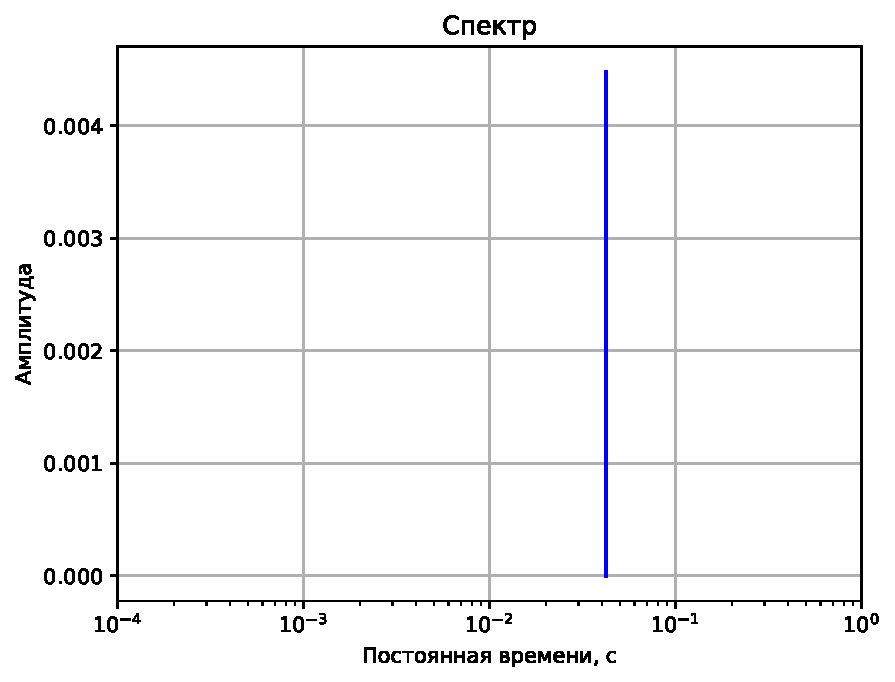
\includegraphics[width=0.75\textwidth]{monoexp_spect_expample}
        \caption{Пример спектра моноэкспоненциального сигнала релаксации
        ёмкости.}
        \label{pic:monoexp_spect_example}
    \end{figure}

    Согласно источнику \cite{istratov_exp_analysis}, зависимость сигнала 
    релаксации ёмкости от времени $f(t)$ для сгинала, образованного 
    несколькими дискретными экспоненциальными сигналами, определяется 
    выражением 
    \ref{eq:discr_multiexp}.
    \begin{equation}
        \label{eq:discr_multiexp}
        f(t) = \sum_{i=1}^{n}A_i\exp\left(-\lambda_i t\right) ,
    \end{equation}
    где $n$ -- количество экспоненциальных составляющих в спектре.
    Пример спектра такого сигнала показан на рисунке 
    \ref{pic:multiexp_spect_example}.
    \begin{figure}[h!]
        \centering
        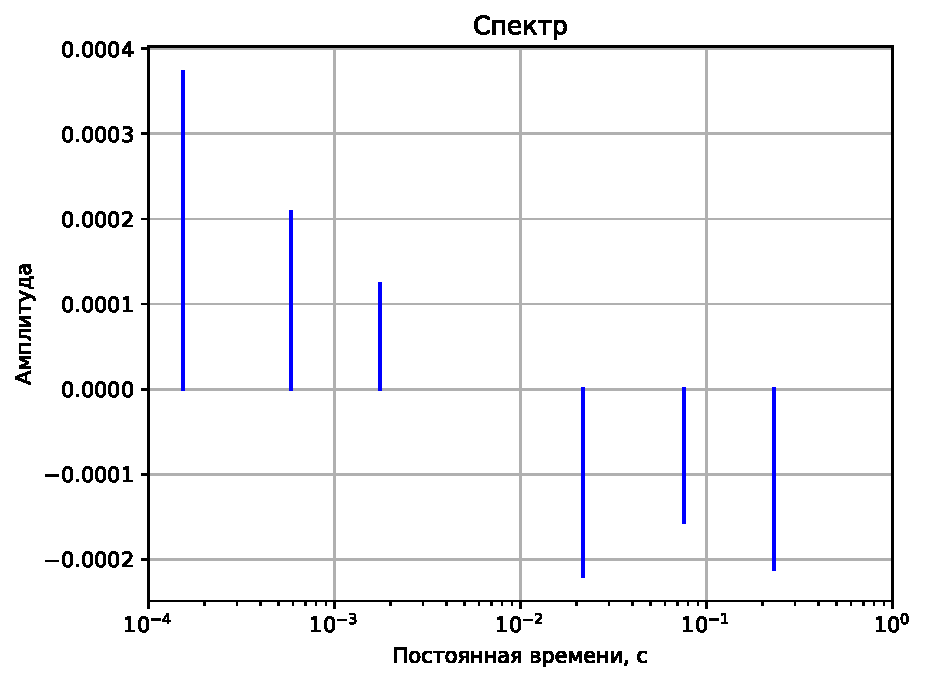
\includegraphics[width=0.75\textwidth]{multiexp_spect_example}
        \caption{Пример спектра сигнала релаксации ёмкости, содержащего
        несколько экспоненциальных составляющих.}
        \label{pic:multiexp_spect_example}
    \end{figure}


    \subsection{Модель аппаратных преобразований спектрометра DLS"~82E}

    В спектрометре DLS-82E реализована корреляционная обработка сигнала
    релаксации ёмкости, таким образом сигнал на выходе аналогового тракта
    спектрометра определяется выражением \ref{eq:dlts_correlation_tech},
    согласно публикации \cite{istratov_exp_analysis}.
    \begin{equation}
        \label{eq:dlts_correlation_tech}
        S\left[g(\lambda),t_c,t_d\right]=\frac{1}{t_c}\int_{t_d}^{t_d+t_c}
        f(t)W\left(t-t_d\right)dt ,
    \end{equation}
    где
    \begin{description}
        \item[$W(t)$] -- весовая функция, определённая на интервале 
        времени $\left[0,t_c\right]$,
        \item[$t_c$] -- период (длительность) весовой функции $W(t)$,
        \item[$t_d$] -- время задержки между началом сигнала релаксации
        и началом корреляционной обработки. Согласно обзору 
        \cite{istratov_exp_analysis}, время задержки $t_d$, обычно, 
        вводится для улучшения избирателности или для снижения искажения
        сигнала из-за перегрузки измерительной системы.
        \item[$g(\lambda)$] -- распределение скоростей экспоненциальных
        спадов, составляющих релаксационный сигнал.
    \end{description}

    Модель аппаратных преобразований (корреляционной обработки),
    учитывающая форму весовой функции, реализованной в спектрометре
    DLS"~82E, для моноэкспоненциального сигнала определяется выражением
    \ref{eq:dls82e_model_S} \cite{rp_vak}.
    \begin{equation}
        \label{eq:dls82e_model_S}
        S\left(\tau,C_A,F_0, t_1\right) = C_A K_{BS} K_{LS} 
        \phi\left(\tau,F_0,t_1\right),
    \end{equation}
    где
    \begin{description}
        \item[$C_A$] -- амплитуда емкостного релаксационного сигнала,
        \item[$K_{BS}$] -- масштабный коэффициент, зависящий от 
        чувствительности емкостного моста,
        \item[$K_{LS}$] -- масштабный коэффициент селектора,
        \item[$\tau$] -- постоянная времени релаксации гулбокого уровня,
        \item[$F_0$] -- частота сканирования импульсов заполнения,
        \item[$t_1$] -- длительность импульса заполнения,
        \item[$\phi\left(\tau,F_0,t_1\right)$] -- функция определяемая
        выражением \ref{eq:dls82e_model_phi}.
    \end{description}
    \begin{equation}
        \label{eq:dls82e_model_phi}
        \phi\left(\tau,F_0,t_1\right) = 
        M \tau F_0 e^{-\frac{0.05}{\tau F_0}}
        \left(1-e^{\frac{t_1 F_0-0.45}{\tau F_0}}
        -e^{-\frac{0.5}{\tau F_0}}+
        e^{\frac{t_1 F_0-0.95}{\tau F_0}}\right),
    \end{equation}
    где $M$ -- масштабный множитель.

    Масштабный множитель $M$ определяется выражением
    \ref{eq:dls82e_model_M}.
    \begin{equation}
        \label{eq:dls82e_model_M}
        M(\tau, F_0, t_1) = \frac{1}{\max{\left[
        \tau F_0 e^{-\frac{0.05}{\tau F_0}}
        \left(1-e^{\frac{t_1 F_0-0.45}{\tau F_0}}
        -e^{-\frac{0.5}{\tau F_0}}+
        e^{\frac{t_1 F_0-0.95}{\tau F_0}}\right)
        \right]}}
    \end{equation}

    Введём коэффициент $A$ (выражение \ref{eq:dls82e_model_A}), 
    характеризующий амплитуду сигнала релаксации ёмкости и перепишем 
    выражение \ref{eq:dls82e_model_S} с учётом того, что длительность
    импульса заполнения $t_1$ является неизменной величиной, и получим
    выражение \ref{eq:dls82e_model_S_short}.
    \begin{equation}
        \label{eq:dls82e_model_A}
        A = C_A K_{BS} K_{LS}.
    \end{equation}
    \begin{equation}
        \label{eq:dls82e_model_S_short}
        S(\tau,A,F_0) = A\phi(\tau, F_0)
    \end{equation}

    Для одновременного учёта нелинейности аппаратного тракта и 
    неэкспоненциальности сигнала релаксации, связанной с присутствием 
    нескольких экспоненциальных составляющих в модель вводят коэффициент
    нелинейности"=неэкспоненциальности $p$ \cite{rp_vak}, после чего 
    выражение \ref{eq:dls82e_model_S_short} приобретает вид выражения 
    \ref{eq:dls82e_model_S_p}.
    \begin{equation}
        \label{eq:dls82e_model_S_p}
        S(\tau,A,F_0,p) = A\left[\phi(\tau, F_0)\right]^p.
    \end{equation}

    Для моноэкспоненциальных сигналов релаксации коэффициент $p=1$, но,
    как будет показано далее, в случае наличия нескольких экспоенециальных
    составляющих в сигнале релаксации коэффициент $p$ становится меньше~1.


    \subsection{Модель для расчёта исходных данных}
    Если предположить, что сигнал релаксации ёмкости состоит из нескольких
    экспоненциальных составляющих и определяется выражением
    \ref{eq:discr_multiexp}, то опираясь на выражения
    \ref{eq:discr_multiexp}, \ref{eq:dlts_correlation_tech}, 
    \ref{eq:dls82e_model_S_short} и \ref{eq:dls82e_model_phi}, можно
    сделать выод, что частотный скан, созданный таким сигналом релаксации
    ёмкости определяется выражением~\ref{eq:multiexp_frequncy_scan}.
    \begin{equation}
        \label{eq:multiexp_frequncy_scan}
        Y = \sum_{i=1}^{n} A_i \phi(\tau_i, F_0) ,
    \end{equation}
    где $n$ -- количество экспоненциальных составляющих в сигнале 
    релаксации.